\documentclass[../../tc_tp5_main.tex]{subfiles}

\begin{document}

%capítulo
\chapter{Celda Universal}

Las celdas universales, son filtros que basan su funcionamiento en etapas de integradores, derivadores y sumadores. Permitiendo crear circuitos de segundo orden.

\begin{figure}[H]	
	\centering
	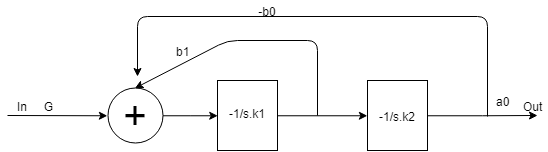
\includegraphics[width=0.6\textwidth]{imagenes/uniGen.png}
	\caption{Cel universal generica}\label{fig:unigen}
\end{figure}

La figura \ref{fig:unigen} muestra una primera aproximación a una celda universal, cuya función transferencia es la siguiente:
$$ H(S)=\frac{S^2 K_1 K_2 }{S^2 K_1 K_2 + b_1 S K_2 + b_0 }$$
de la ecuación se obtiene $Q$ y $W_0$:

$$W_0=\sqrt{\frac{b_0}{K_1 K_2}}$$
$$Q=\frac{1}{b_1}\sqrt{\frac{b_0 K_1}{K_2}}$$

Las sensibilidades de $Q$ y $W_0$ son:
$$ S^{W_0}_{b_0}=\frac{ \partial W_0}{\partial b_0} \frac{b_0}{W_0}= \frac {1}{2}$$

$$ S^{W_0}_{K_1}= S^{W_0}_{K_2}= - S^{W_0}_{b_0}= \frac {-1}{2}$$

$$ S^{Q}_{b_0}=\frac{ \partial Q}{\partial b_0} \frac{b_0}{Q}= \frac {1}{2}$$

$$ S^{Q}_{K_1}= S^{Q}_{K_2}= S^{Q}_{b_0}= \frac {1}{2}$$

\clearpage\newpage


\end{document}
